\documentclass{article}
\renewcommand\refname{Referencias}
\renewcommand\contentsname{\'Indice de Conten\'ido}
\usepackage{graphicx}
\graphicspath{{../../IMG/}}
\usepackage{caption}
\usepackage{subcaption}
\usepackage{float}
\usepackage{listings}

\title{\textsc{Paradigmas y Lenguajes de Programaci\'on\\Gu\'ia TP - Unidad 1}\\\textit{Diapositiva}}
\author{Ulises C. Ramirez}
\date{12 de Septiembre, 2018}

\begin{document}
\maketitle
\pagenumbering{gobble}
\newpage
\section*{Versionado}
Para el corriente documento se est\'a llevando un versionado a fin de mantener un respaldo del trabajo y adem\'as proveer a la c\'atedra o a cualquier interesado la posibilidad de leer el material en la \'ultima versi\'on disponible.\\

\textsc{Repositorio}: \textit{https://github.com/ulisescolina/UC-PYLP}

\tableofcontents
\pagenumbering{gobble}
\newpage

% === Inicio del Cuerpo del Documento === %
\pagenumbering{arabic}
\section{Ejercicio 1}
\label{sec:e1}
\subsection{?`Qu\'e diferencia existe entre la multiprogramaci\'on y el multiproceso?}
Ambos describen una forma de compartir el tiempo de computo de un sistema por programas, que en ultima instancia ayuda a dar una explicaci\'on conceptual de lo que significa concurrencia. La diferencia la expuesta en \cite{gortazarbellas} es la siguiente:
La \textbf{\textit{Multiprogramacion}}, se da cuando los programas se ejecutan en un \'unico procesador disponible y sus procesos internos comparten el tiempo de c\'omputo del procesador mencionado. Se habla de \textbf{\textit{Multiproceso}}, cuando el sistema en el cual se ejecuta el programa posee multiples procesadores, entonces es posible asignar diferentes procesos a diferentes procesadores.

\subsection{?`Qu\'e es una \textit{instrucci\'on at\'omica} y que es la \textit{intercalaci\'on}?}
\label{sub:atomicaintercalacion}
Se considera una \textit{instrucci\'on at\'omica} \cite{gortazarbellas} a aquella que se ejecuta completamente antes de que se ejecute ninguna otra instrucci\'on de cualquier otro proceso del programa, una \textit{intercalaci\'on} en un programa es una secuencia de ejecuci\'on de las instrucciones at\'omicas con las que cuente dicho programa, en el caso de que hayan 2 instrucciones at\'omicas ejecutadas por 2 procesos concurrentes, existiran 4 posibles intercalaciones.

\subsection{?`Considera que \texttt{a:=a+1} una instrucci\'on at\'omica? Justifique la respuesta}
Para dar respuesta a \'esta pregunta es necesario saber, como se especif\'ica en \cite{gortazarbellas}, \textit{qu\'e instrucciones del lenguaje son realmente instrucciones at\'omicas}, para \'esto debemos saber primero de que lenguaje de programaci\'on se esta hablando a la hora de responder a la consigna, para propositos pr\'acticos se asume que se trata de PascalFC.
La siguiente tabla, extra\'ida de la cita realizada en \'esta secci\'on, indica cuales son las instrucciones que debe realizar el lenguaje para realizar \texttt{a:=a+1}.
\begin{figure}[H]
  \centering
  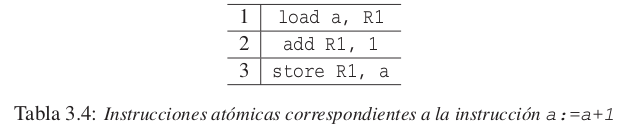
\includegraphics[width=.5\linewidth]{a+1.png}
  \label{fig:a1}
\end{figure}
Primero se carga el valor de \texttt{a} en el registro \texttt{R1}, acto seguido se procede a realizar la suma de lo que se encuentra cargado en el registro y la constante prove\'ida, en este caso el valor 1 y se procede a guardar el resultado en el registro \texttt{R1}, y en \'ultima instancia se asigna lo que se tiene en \texttt{R1} a \texttt{a}.

\subsection{?`Qu\'e podr\'ia pasar si dos procesos ejecutaran en paralelo la instrucci\'on \texttt{a:=a+1}?}
Las instrucciones at\'omicas que se discutieron en la \texttt{Subsecci\'on \ref{sub:atomicaintercalacion}} se pueden aplicar al problema \texttt{a:=a+1}, de esta manera las instrucciones at\'omicas que conformar\'ian la operacion serian las mencionadas en la \texttt{Figura \ref{fig:a1}}, entonces lo que puede suceder si dos procesos ejecutan de manera concurrente el mismo bloque con la variable compartida \texttt{a} los resultados podr\'ian ser imprevistos, dado al fenomeno de la intercalaci\'on.

\section{Ejercicio 2}

\textsc{Consigna}: \textbf{investigar como instalar el lenguaje PascalFC en su sistema operativo. Lectura recomendada por la c\'atedra: p\'agina del Ing. John Coppens \textit{http://jcoppens.com/soft/pfc2}}

\section{Ejercicio 3}
\label{sec:e3}
\textsc{Consigna}: \textbf{\begin{itemize}
\item Implemente el ejercicio de la diapositiva 10 en PascalFC.
\item Al ejecutarlo varias veces, ?`Qu\'e sucede con la salida del mismo?
\end{itemize}}

\section{Ejercicio 4}
\textsc{Consigna}: \textbf{investigar: \begin{itemize}
\item ?`Qu\'e son los sem\'aforos en la programaci\'on paralela?
\item ?`Para qu\'e sirven?
\item ?`Cu\'ales son sus instrucciones y para qu\'e se utiliza cada una?
\end{itemize}}
\subsection{?`Qu\'e son los sem\'aforos en la programacion paralela?}
Los sem\'aforos son una herramienta que se destina para la sincronizaci\'on de procesos, en PascalFC estos son un tipo abstracto de datos, y como tal tiene operaciones y estructuras de datos internos. Todo sem\'aforo tiene un contador que toma valores positivos, y una lista de procesos asociados.
\subsection{?`Para qu\'e sirven?}
Estos sirven para garantizar que recursos en el sistema que deben ser utilizados por un proceso a la vez, efectivamente sean utilizados por un proceso a la vez, este conjunto de instrucciones que acceden a las areas mencionadas son denominados \textit{secci\'on cr\'itica}.

\subsection{?`Cuales son sus instrucciones y para que se utiliza cada una?}
Las operaciones que se pueden invocar sobre una variable de tipo sem\'aforo son:
\begin{itemize}
\item \texttt{initial(s,v)} inicializa el contador del sem\'aforo \texttt{s} al valor \texttt{v}. Este procedimiento solo se puede invocar una vez y debe ser llamado desde el programa principal. Debe ser inicializado antes de utilizarse.
\item \texttt{wait(s)} Este procedimiento solo se puede invocar desde un proceso. Funcionamiento:
  \begin{itemize}
    \item Si el contador \texttt{s} tiene un valor mayor que cero, el proceso contin\'ua su ejecuci\'on y el valor del contador se decrementa en uno.
    \item Si el contador del sem\'aforo tiene el contador igual a cero, el proceso se queda bloqueado y se a\~{n}ade a la lista de procesos bloqueados del sem\'aforo.
  \end{itemize}
\item \texttt{signal(s)} Este procedimiento solo se puede invocar desde un proceso. Funcionamiento:
  \begin{itemize}
    \item Si no hay procesos bloqueados en el sem\'aforo \texttt{s}, se incrementa el valor de contador en una unidad.
    \item Si hay procesos bloqueados en el sem\'aforo, se elige aleatoriamente a uno de ellos y se desbloquea para que continue su ejecuci\'on.
  \end{itemize}
\end{itemize}



\section{Ejercicio 5}
\textsc{Consigna}: \textbf{investigue e implemente una solucion en PascalFC con sem\'aforos al problema de la salida detectada en el \texttt{Ejercicio \ref{sec:e3}}.}


% === Bilbiografia === %

\begin{thebibliography}{99}
	% Item 1
	\bibitem[Gort\'azar Bellas, et al, 2012]{gortazarbellas}\textsc{Gort\'azar Bellas, Francisco; Mart\'inez Unanue, Raquel; Fresno Fern\'andez, Victor}. \textit{Lenguajes de Programaci\'on y Procesadores - Cap\'itulo 3.5}. Editorial Universitaria Ramon Areces, Madrid, 2012. \textsc{ISBN: 9788499610702}.
\end{thebibliography}
\end{document}
